\documentclass[a4paper,11pt]{article}
\usepackage[margin=2cm]{geometry}
\geometry{a4paper}  
\usepackage[T1]{fontenc}
\usepackage[utf8]{inputenc}
\usepackage{lmodern}
\usepackage{amsmath}
\usepackage{amsfonts}
\usepackage{amssymb}
\usepackage{graphicx}


\title{Homology Benchmark}
\author{Jacob Joseph, Adrian Altenhoff}

\begin{document}

\maketitle

This text briefly summarizes the Homology Test contributed by Dannie Durand and Jacob Joseph.

The following figure shows a homologous family (black dots enclosed in circle). 
\begin{figure}[hbt]
  \begin{center}
    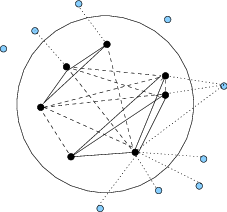
\includegraphics[width=.5\textwidth]{figures/homologyBenchmark}
    \label{fig}
  \end{center}
\end{figure}

Orthologs are connected by solid lines. Paralogs are connected by dashed lines. Dotted lines indicate significant similarity to unrelated
sequences (blue dots) due to shared promiscuous domains, convergent evolution, chance similarity, etc. Our
data set is designed to evaluate the ability of a method to separate pairs of black dots (homologous pairs, whether orthologs and paralogs) from pairs containing one blue dot and one black dot (non-homologous pairs).

In the context of ortholog prediction, the currated dataset of multidomain homologs can be used to evaluate whether similar, but non-homologous pairs (blue, black) are mis-identified as orthologs. It is \emph{not} useful for testing whether paralogs (dashed lines) are mis-identified as orthologs (solid lines). Moreover, if we use the positive and negative pairs in our data set ``as is'', without modification, the failure to report paralogous pairs as true positives would be penalized. This is inappropriate in this case, since the goal in ortholog prediction is just the opposite, namely to exclude them. We need a way to correct for that. So, here’s what we do:

Let $Z = {(z1 , z2 ),\ldots}$ be a set of ortholog predictions. Further, let $X = {(x1 , x2 ), \ldots}$ be the set of known positives and $Y = {(x1 , y1 ), \ldots}$ be the set of known true negatives in our curated data. We restrict both $X$ and $Y$ to include mouse-human pairs---the covered set of species of this dataset---only.

Further let
$Z^{'} = Z \cap (X \cup Y )$
be the set of predicted pairs in $Z$ for which we have annotation information. In other words, we exclude
sequences from families or genomes that we have not curated from further analysis.

As a proxy for the sensitivity of each method, we report the \textbf{coverage} of the predicted orthologs of the cureated dataset.
$$Cov = |(Z^{'} \cap X )|.$$
In other words, $Cov$ is the number of predictions that (1) are within the annotated set and (2) are known positives. Additionally, we report the \textbf{False Discovery Rate} 
$$FDR = |(Z^{'} \cap Y )| / |Z^{'}|.$$
This is the fraction of predictions that (1) are within our annotated set and (2) are known negatives.

Note that it is not valuable to use the curated dataset to assess sensitivity/recall in its proper context, since our set contains many paralogous pairs that we consider true positives, but are negatives for the purposes of orthology prediction.

\end{document}
